\section{Reachability Analysis of Finite State Machines (FSMs) using Algebraic Geometry}
% \subsection{An example illustrating our proposed approach}
In our approach we use symbolic state reachability with algebraic
geometry concepts. It is an abstraction based on word operand
definition of datapaths in circuits, and it can be applied
to arbitrary FSMs by bundling a set of bit-level variables together as
one or several word-level variables.  The abstraction polynomial,
encoding the reachable state space of the FSM, is obtained through
computing a GB of an elimination ideal using elimination term order
based on theorem \ref{thm:elim}.  

The motivation behind our approach can be described as follows:
\begin{itemize}
\item Any finite set of points is the variety (solutions) of a
  polynomial ideal. Since the state-space of a FSM is finite, it can
  be construed as the variety of an ideal corresponding to the
  function (circuit implementation, gates) of the   sequential circuit.
\item Using canonical representations of polynomial ideals (Gr\"obner
  bases), the transition functions and the sets of states can be used
  for FSM traversal and property checking. 
\item In our work, Gr\"obner bases are considered in lieu of BDDs or
  SAT-solvers. Furthermore, instead of working in the Boolean domain
  $\B$, we model the circuit and the properties over the Galois field
  $\Fkk$. This allows to perform reachability analysis at the level of
  $k$-bit words, as $\mathbb{F}_2 \subset \Fkk$.

\end{itemize}

Reachability analysis is a useful tool when checking sequential
equivalence as well as other invariants. 
%With word-level state
%variables, we can do implicit state enumeration to provide a picture
%of  reachable states. 
Conceptually, the state-space of a FSM is traversed in a breadth-first
manner, as shown in Algorithm \ref{alg:BFS}. % \cite{KallaPartialScan}: 
In general, the algorithm operates on the FSM 
$\mathcal{M} = (\sum, O, S, S^0, \Delta, \Lambda)$ underlying a
sequential circuit. In such cases, the transition function $\Delta$
and the initial states are represented and manipulated using Boolean
representations such as BDDs or SAT solvers. The variables $from,
reached, to, new$ represent characteristic functions of sets of
states. Starting from the initial state $from^i = S^0$, the algorithm
computes the states reachable in 1-step from $from^i$ in each iteration.
In line 4 of algorithm \ref{alg:BFS}, the {\bf image computation} is
used to compute the 1-step next reachable states. In
\cite{KallaPartialScan}, the author implicitly represents the states
and transition relations by Boolean functions and Boolean vectors,
respectively. 


Let us describe the application of the algorithm on the  FSM circuit
of Fig.\ref{fig:fsm}. {\it We will first describe its operation at the
Boolean level, and then describe how this algorithm can be implemented
using algebraic geometry at word level.} 


In Line 1 of the BFS algorithm, assume that the initial state
is $S_3$ in Fig.\ref{fig:fsm}(b), which is encoded as 
$S_3 = \{11\}$. Using Boolean variables $s_0, s_1$ for the present
states, $from^0 = s_0\cdot s_1$ is represented as a Boolean formula. 


The {\it transition function} $\Delta$ is given by Boolean equations
  of the flip-flops of the circuit: $t_i = \Delta_i(s, x)$, where
  $t_i$ is the next state variable, $s$ represents the present   state
  variables and $x$ represents the input variables. 
The {\it Transition relation of the FSM} is then represented as: 
\begin{equation} 
T(s, x, t) =   \prod_{i=1}^{n} (t_i \overline{\oplus } \Delta_i)
\end{equation}
where $n$ is the number of flip flops, and $\overline{\oplus}$ is XNOR
operation. Let $from$ denote the set of initial states, then the
image of the initial states, under the transition function $\Delta$ is
finally computed as:
\begin{align}
\label{img}
to = \text{Img}(\Delta, from) = \exists _s ~\exists _x ~[ T(s, x, t)
  \cdot from ] = \exists _s ~\exists _x ~\prod_{i=1}^{n} (t_i
\overline{\oplus } \Delta_i)\cdot from
\end{align}

Here, the notation $\exists x (f)$ represents the {\it existential
  quantification of $f$ w.r.t. variable $x$}. 

\begin{algorithm}[hbt]
\SetAlgoNoLine
 \KwIn{Transition functions $\Delta$, initial state $S^0$}

  $from^0 = reached = S^0$\;
  \Repeat{$new^i == 0$}
  {
  	$i \gets i + 1$\;
	$to^i \gets$Img$(\Delta, from^{i-1})$\;
	$new^i \gets to^i \cap \overline{reached}$\;
  	$reached \gets reached \cup new^i$\;
	$from^i \gets new^i$\;
  }
\Return{$reached$}
\caption {Breadth-first Traversal Algorithm for Reachability Analysis of FSMs}\label{alg:BFS}
\end{algorithm}


\begin{example}
For the circuit in Fig. \ref{fig:fsm} (b), we have the transition
functions of the machine as:

\begin{align*}
\Delta_1: & ~t_0 \overline{\oplus} ((\overline{x + s_0 + s_1}) + s_0 s_1)\\
\Delta_2: & ~t_0 \overline{\oplus} (\overline{s_0}x + \overline{s_1}s_0)\\
from:     & ~from^0 = s_0\cdot s_1
\end{align*}



When the formula of Eqn. (\ref{img}) is applied to compute 1-step
reachability, $to = \exists _{s_0, s_1, x} (\Delta_1 \cdot \Delta_2
\cdot from^0)$, we obtain $to = \overline{t_0}\cdot t_1$, which denotes
the state $S_1 = \{01\}$ reached in 1-step from $S_3$.

In the next iteration, the algorithm uses state $S_1 = \{01\}$ as the
current (initial) state, and computes $S_2 = \{10\} = t_0\cdot
\overline{t_1}$ as the next reachable state, and so on. 
\end{example}

%% Let  $\Delta_i$ denote the transition function for $i^{th}$ bit of the
%% output $T$
%% (denoted by $t_i$), and it is described by a Boolean function. We can
%% obtain the transition relation  for bit-vector $T$:
%% $Tran(s_0,s_1,x,t_0,t_1) =
%% \bigwedge_{i=1}^{2}(t_i\ \bar{\oplus}\ \Delta_i)$. Assume present
%% states are represent by Boolean formulas $PS(s_0,s_1)$, then the image
%% function is written as $\text{Img}(Tran,\ PS) =
%% \exists_{s_0,s_1}\exists_{x}[Tran(s_0,s_1,x,t_0,t_1)\land
%%   PS(s_0,s_1)]$, where $\exists_x f$ denotes the existential
%% quantification of $f$ w.r.t. $x$. 

Our objective is to model the transition functions $\Delta$ as a
polynomial ideal $J$, and to perform the image computations (Algorithm
\ref{alg:BFS}, line 4) using Gr\"obner bases over Galois fields. {\bf
This requires to perform quantifier elimination; which can be
accomplished using the Gr\"obner basis computation over Galois fields
by using elimination ideals} \cite{gao:qe-gf-gb}. Finally, the set
union,  intersection and complement operations are also to be
implemented in algebraic geometry.

{\bf FSM Traversal at word-level over $\Fkk$:} 
The state transition graph (STG) shown in Fig.\ref{fig:fsm}(a) uses a
2-bit Boolean vector to represent 4 states $\{S_0, S_1, S_2,
S_3\}$. We map these states to elements in $\mathbb{F}_{2^2}$, where
$S_0 = 0, S_1 = 1, S_2 = \alpha, S_3 = \alpha+1$ where $\alpha^2 +
\alpha + 1 = 0$. 

{\it Initial state:} In Line 1 of the algorithm, the initial state is
specified by means of a corresponding polynomial $f = \mathcal{F}(S) =
S - 1 - \alpha$. Notice that if we consider the ideal generated by the
initial state polynomial, $I = \langle f\rangle$, then its variety
$V(I) = 1+\alpha$, corresponds to the state encoding $S_3 = \{11\} =
1+\alpha$, where a polynomial in word-level variable $S$ encodes the
initial state. 
% with only one generator $f$, its variety
% $V(I) = \{\gamma\ |\ \gamma \in \mathbb{F}_{2^2}, \gamma = 1+\alpha\}$, which equals to $\{1+\alpha\}$, the only
% valid value $S_3$ can take.


%Using theorems from Section \ref{sec:elim}, we implement the image
%function by a GB computation on elimination ideal. Ex.\ref{ex:motiv}
%is an example for our implementation of image function, i.e. one-step
%reachability. 

{\bf Set operations:} When executing Line 5 and Line 6, we use
\textbf{union}, \textbf{intersection} and \textbf{complement} of
varieties over $\mathbb{F}_{2^k}$: 

\begin{definition}
\label{def:sum}
({\bf Sum/Product of Ideals}) If $I = \langle f_1, \dots, f_r\rangle$ and $J = \langle g_1, \dots, g_s\rangle$ are 
ideals in $\mathbb F[x_1, \dots, x_n]$, then the {\bf sum} of $I$ and $J$ is defined as
$$I + J = \langle f_1, \dots, f_r, g_1, \dots, g_s\rangle$$ And the {\bf product} of $I$ and $J$ is defined
as
\begin{equation}
  I \cdot J = \langle f_ig_j\ |\ 1 \leq i \leq r, 1 \leq j \leq s\rangle \nonumber
  \end{equation}
\end{definition}

With concepts of ideal sums and products, we can obtain the
intersection and union of affine varieties as:
\begin{theorem}
\label{thm:unionintersect}
If $I$ and $J$ are ideals in $\mathbb F[x_1, \dots, x_n]$, then ${\bf
  V}(I + J) = {\bf V}(I) \bigcap {\bf V}(J)$ and ${\bf V}(I \cdot J) =
{\bf V}(I) \bigcup {\bf V}(J)$. 
\end{theorem}


In Line 5 of Alg.\ref{alg:BFS}, we need to compute the complement of a
set of states. Assume that $J$ denotes a polynomial ideal whose
variety $V(J)$ denotes a set of states. We require the computation of
another polynomial ideal $J'$, such that $V(J') =
\overline{V(J)}$. We have recently proved (the proofs are omitted)
that this computation can be performed using the concept of {\bf ideal
  quotient:} 

\begin{definition}
({\bf Quotient of Ideals}) If $I$ and $J$ are ideals in $\mathbb
  F[x_1, \dots, x_n]$, then $I:J$ is the set
  \begin{equation}
  \{f \in \mathbb F[x_1, \dots, x_n]\ |\ f\cdot g \in I, \forall g \in J\}\nonumber
  \end{equation}
and is called the {\bf ideal quotient} of $I$ by $J$.
\end{definition}


% However, complement of variety cannot be easily dealt by simple arithmetic on polynomial generators.
% For non-trivial cases we can only prove that 
% \begin{theorem}
% Let $I, J$ be ideals in $\mathbb F[x_1,\dots,x_n]$, then 
% $${\bf V}(I:J) \supset {\bf V}({\bf I}({\bf V}(I) - {\bf V}(J)))$$
% \end{theorem}
% Fortunately for most hardware verification cases, the form of polynomial generators are restricted.
% A proposition has been proved by \cite{jinpeng} that after adding {\bf vanishing polynomials ideal}
% the new composed ideal implies following corollary:

For elimination ideals in circuit verification problems, we can obtain
the complement of a variety through the following result:

\begin{theorem}
\label{thm:quotient}
Let $I, J$ be ideals with vanishing polynomials over $\Fkk[x_1,\dots,x_n]$, then 
$${\bf V}(I:J) = {\bf V}(I) - {\bf V}(J)$$
\end{theorem}


Let $J_0 = \langle x_1^{2^k} - x_1, \dots, x_n^{2^k} - x_n \rangle$
denote the ideal of all vanishing polynomials in $\Fkk$. Then, we have
$V(J_0) = (\Fkk)^{n}$; i.e. the variety of vanishing ideal contains
all possible valuations of variables, so it constitutes the {\bf
  universal set}. Subsequently, the {\bf absolute complement} can be
computed as:

\begin{corollary}
$$V(J') = \overline{{\bf V}(J)} = {\bf V}(J_0:J)$$

\end{corollary}

In other words, the ideal $J'$, computed as $J' = J_0:J$ is such that
$V(J') =\overline{V(J)}$. 

Since we can add vanishing polynomials for state sets
$from^i, to^i, reached$, it is feasible to use above corollary. We
will demonstrate the application of this important concept through an
example. 
% 
% {\bf Now, STEP BY STEP, SHOW THE FULL Blown traversal COMPUTATION
%   HERE.... Make sure to also show how elimination order with GB
%   computation is also used...} \vspace{0.5in}


Assume $I = \langle f\rangle  = \langle T^2 +
(1+\alpha)\cdot T+\alpha\rangle $,  we can add vanishing polynomial
$T^4 - T$ to this ideal such that its variety  $V(I) = \{a\ |\ a \in
\mathbb{F}_{2^2}\ and\ f(a) = 0\} = \{1, \alpha\}$. For complement set
of variety $\{1, \alpha\}$, the universal set is the variety of ideal
of vanishing polynomial $V(\langle T^4-T\rangle ) =
\{0,1,\alpha,1+\alpha\}$, 
so $\overline{V(\langle T^2 + (1+\alpha)\cdot T+\alpha\rangle )} = V(\langle T^4-T\rangle ) - V(\langle T^2 + (1+\alpha)\cdot T+\alpha\rangle )$,
which equals to $V(\langle T^4-T\rangle :\langle T^2 + (1+\alpha)\cdot T+\alpha\rangle ) = V(\langle T^2+(1+\alpha)\cdot T\rangle )$,
the result is $\{0,1+\alpha\}$.

According to the discussion above, the BFS traversal can be completely implemented using algebraic geometry.
as in Algorithm \ref{alg:univa}.

\begin{algorithm}[hbt]
\SetAlgoNoLine
 \KwIn{Input-output circuit characteristic polynomial ideal $J_{ckt}$, initial state polynomial $\F(S)$}

  $from^0 = reached = \F(S)$\;
  \Repeat{$new^i == 1$}
  {
  	$i \gets i + 1$\;
	$to^i \gets$GB w/ elimination term order$\langle J_{ckt},J_0, from^{i-1}\rangle$\;
	$new^i \gets $generator of $\langle to^i\rangle + (\langle T^4-T\rangle:\langle reached\rangle)$\;
  	$reached \gets $generator of $\langle reached\rangle \cdot \langle new^i\rangle$\;
	$from^i \gets new^i(S\setminus T)$\;
  }
\Return{$reached$}
\caption {Algebraic Geometry based Traversal Algorithm}\label{alg:univa}
\end{algorithm}

Here $from^i, to^i, new^i$ are all univariate polynomials in variables $S$ or $T$, due to GB computation
with elimination term order.

\begin{example}
We apply Algorithm \ref{alg:univa} to Ex.\ref{ex:motiv} to execute the FSM traversal. Let the initial state
$from^0 = S$ (i.e. state $\{00\}$), in the first iteration we compose an elimination ideal $J$ with

\begin{minipage}[h]{0.4\textwidth}
\begin{align*}
&f_1: t_0- (xs_0s_1+xs_0+xs_1+x+s_0+s_1+1)\\
&f_2: t_1 - (xs_0+x+s_0s_1+s_0)\\
&f_3: S - s_0 - s_1\\
&f_4: T - t_0 - t_1
\end{align*}
$J_{ckt} = \langle f_1,f_2,f_3,f_4\rangle$
\end{minipage}
\begin{minipage}[h]{0.6\textwidth}
\begin{align*}
&f_5: x^2-x\\
&f_6: s_0^2-s_0, ~~f_7: s_1^2-s_1\\
&f_8: t_0^2-t_0, ~~~f_9: t_1^2-t_1\\
&f_{10}: S^4-S, ~f_{11}:T^4-T
\end{align*}
$\ \ \ \ \ \ \ \ \ \ \  \ J_0 = \langle f_5,f_6,\dots,f_{11}\rangle$
\end{minipage}

and $from^0$. Compute the reduced GB for $J = J_{ckt}+J_0+\langle from^0\rangle$,
with elimination term order
$$\{x,s_0,s_1,t_0,t_1\}~(all~PI~and~bit~level~variables)~>~S~(PS~word)~ >~ T~(NS~word)$$
the result contains
a polynomial generator with only $T$, we assign it to next state $$to^1 = T^2+(\alpha+1)T+\alpha$$ denoting
$\{01,10\}$. Since formerly reached state $reach = T$, its complement is $$\langle T^4-T\rangle:\langle T\rangle
= T^3+1$$ (i.e. states $\{01,10,11\}$). Then the newly reached state in this iteration is
$$\langle T^3+1, T^2+(\alpha+1)T+\alpha \rangle = \langle T^2+(\alpha+1)T+\alpha \rangle$$ We add these states
to formerly reached states $$reach = \langle T\cdot T^2+(\alpha+1)T+\alpha \rangle = \langle T^3+(\alpha+1)T^2+\alpha T\rangle$$
(i.e. states $\{00,01,10\}$). We update the present states for next iteration $$from^1 = S^2+(\alpha+1)S+\alpha$$

In the second iteration, we compute the reduced GB with the same term order for ideal $J = J_{ckt}+J_0+\langle from^1\rangle$.
It includes a polynomial generator $$to^2 = T^2+\alpha T$$ denotes states
$\{00,10\}$. The complement of $reached$ is $$\langle T^4-T\rangle:\langle T^3+(\alpha+1)T^2+\alpha T\rangle
= T + 1+\alpha$$ (i.e. states $\{11\}$). We compute the newly reached state 
$$\langle T^2+\alpha T, T+1+\alpha \rangle = \langle 1\rangle$$ 
It means the newly reached state is empty, thus a fixpoint has been detected. The algorithm terminates and returns
$$reached = \langle T^3+(\alpha+1)T^2+\alpha T\rangle$$ as final reachable states.

% 
% $J = \langle t_0- (xs_0s_1+xs_0+xs_1+x+s_0+s_1+1), t_1 - (xs_0+x+s_0s_1+s_0), S - s_0 - s_1, T - t_0 - t_1, S \rangle$
% and a vanishing polynomial ideal $J_0 = \langle x^2-x, s_0^2-s_0, s_1^2-s_1, t_0^2-t_0, t_1^2-t_1, S^4-S, T^4-T\rangle$
% The elimination term order is $\{x,s_0,s_1,t_0,t_1\} > S > T$. Compute a reduced GB for $J+J_0$, the result has 
% a polynomial generator with only $T$, we assign it to next state $to^1 = T^2+(\alpha+1)T+\alpha$ denoting
% $\{01,10\}$. Since formerly reached state $reach = T$, its complement is $\langle T^4-T\rangle:\langle T\rangle
% = T^3+1$ (i.e. states $\{01,10,11\}$). Then the newly reached state in this iteration is
% $\langle T^3+1, T^2+(\alpha+1)T+\alpha \rangle = \langle T^2+(\alpha+1)T+\alpha \rangle$. We add these states
% to formerly reached states $reach = \langle T\cdot T^2+(\alpha+1)T+\alpha \rangle = \langle T^3+(\alpha+1)T^2+\alpha T\rangle$
% (i.e. states $\{00,01,10\}$). We update the present states for next iteration $from^1 = S^2+(\alpha+1)S+\alpha$.
% In the second iteration, we just replace 1 generator in $J+J_0$: $S$ with $S^2+(\alpha+1)S+\alpha$, and elimination
% term order keeps the same. The reduced GB includes a polynomial generator $to^2 = T^2+\alpha T$ denotes states
% $\{00,10\}$. The complement of $reached$ is $\langle T^4-T\rangle:\langle T^3+(\alpha+1)T^2+\alpha T\rangle
% = T + 1+\alpha$ (i.e. states $\{11\}$). We compute the newly reached state 
% $\langle T^2+\alpha T, T+1+\alpha \rangle = \langle 1\rangle$, then the algorithm terminates and returns
% $reached = \langle T^3+(\alpha+1)T^2+\alpha T\rangle$ as final reachable states.
\end{example}

{\bf Significance for using GB:} Reduced GB is a unique, minimal and
{\bf canonical} representation of the circuit's function. Starting
from a certain initial state and using a reduced GB to represent the
transition function, reachable states can be computed and represented
canonically. Then it becomes possible to identify  when a fixpoint
is reached (termination of the algorithm) by performing an equality
check of polynomial ideals. 

\subsection{Research objective: To make the approach scalable}

At the time of writing this proposal, the theoretical concepts behind
the word-level FSM traversal have been studied and validated. A
completed algorithm has been devised and preliminary experiments were
conducted for reachability analysis using the {\sc Singular} computer
algebra tool \cite{DGPS}. While the approach is shown to work
correctly and completely, it is practically infeasible. The complexity
lies in the Gr\"obner basis computation. 

Over Galois fields of the type $\Fkk$, computing the reduced Gr\"obner
basis of the ideal $(J + J_0)$ requires both memory and space
${2^{k}}^{O(n)}$; where $J$ is an arbitrary polynomial ideal, $J_0$ is
the vanishing ideal, and $n$ is the number of variables in the system
(circuit). In this research, I wish to draw inspirations from the work
of \cite{jinpeng} and \cite{timDAC} to overcome the
complexity of GB computations. 


In \cite{jinpeng}, the authors analyze the given circuit topology,
and derive a term order to represent the polynomials. They show that
this term order renders the set of polynomials itself a Gr\"obner
basis of the ideal. In \cite{timDAC}, the authors use a similar
concept to derive a {\it refinement of the abstraction term order}
(RATO) to simplify the Gr\"obner basis computation. However, the above
concepts are applied to combinational circuit verification. I will
investigate how similar techniques can be explored for the
computations that are needed in Algorithm \ref{alg:univa} for
reachability analysis to make the approach scalable. I believe that it
is possible to make the approach scalable, as I have recently
demonstrated in a paper \cite{myDATE} %{\bf refer to the DATE paper here?}
which has been accepted for publication at the {\it Design Automation
  and Test in Europe Conference}, 2015. 



\subsection{Research objective : Application to Unrolling Sequential Circuits for Sequential Arithmetic Verification}
In above discussions, we propose an implicit state enumeration algorithm implemented by GB computations over
an elimination ideal, which is usually applied on FSMs working as control units. For many arithmetic
datapath components, state enumeration is not the best way to verify the function of circuit. On the one hand, the signals preloaded
to the state variables in FSM are usually not specified such that we can hardly encode the initial states; on the other
hand, instead of the set of globally reachable states, arithmetic verification focuses on exact reached states
after $k$ clock cycles which reflects desired arithmetic function. Considering these reasons, we modify
our algebraic geometry based approach and apply it to implicit FSM unrolling. 

% In above discussions, we propose an implicit state enumeration algorithm implemented by GB computation over
% an elimination ideal, which is usually applied on Mealy FSMs working as control unit. For many arithmetic
% datapath components, they should be modeled as Moore FSMs according to their structures. On the one hand, the signals preloaded
% to a Moore FSM are usually not specified such that we can hardly encode the initial states; on the other
% hand, instead of the set of globally reachable states, arithmetic verification focuses on exact reached states
% after $k$ clock cycles which reflects desired arithmetic function. Considering these reasons, we modify
% our algebraic geometry based approach and apply it to Moore FSM unrolling. 

% % Figure Moore.eps
% \begin{figure}[hbt]
% \centering{
% %\begin{minipage}{12cm}
% 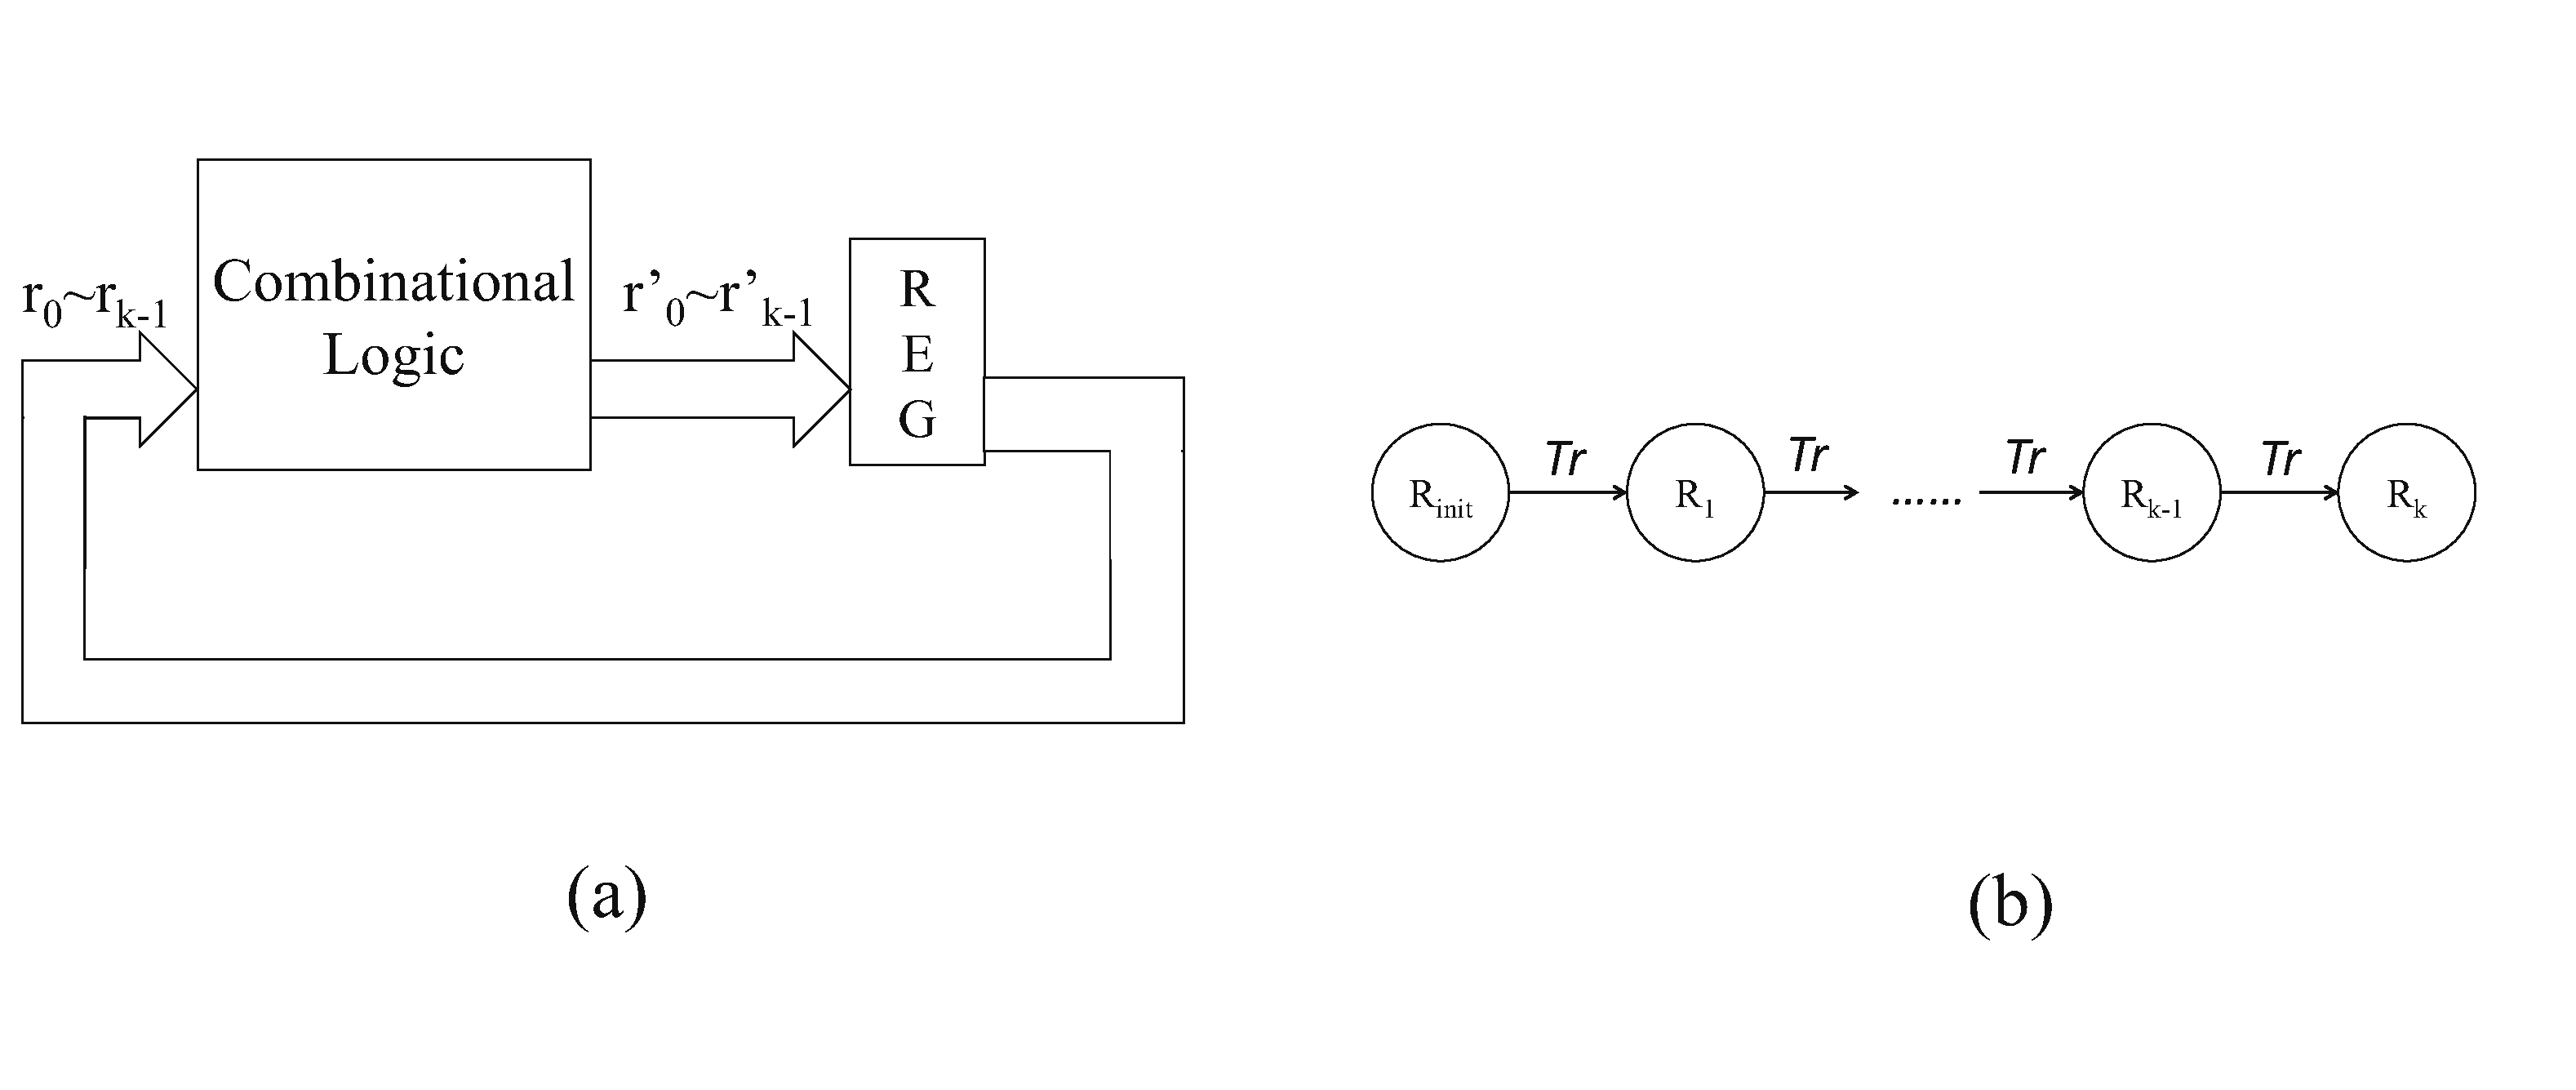
\includegraphics[width=7.5in]{./Moore.eps}
% % \vspace{-0.2in}
% \caption{A simple Moore FSM and its state transition graph}
% %\end{minipage}
% \label{fig:Moore}}
% \end{figure}

Fig.\ref{fig:seqmodel}(b) shows a typical Moore FSM without primary inputs, $R$ is the word-level state variable. Let word-level indeterminate 
$R_{init}$ denote the initial preloaded value of $R$, and $R_{i}$ denote the evaluation of $R$ after $i$ clock cycles
(transitions). Transition relation $Tr:R_{i-1}\to R_i$ can be modeled similar to
the image function in Algorithm \ref{alg:BFS}. Assume that after $k$ clock cycles, the machine should give a state output
$R_{k} = \mathcal F(R_{init})$. To verify this result, we can implicitly unroll this FSM and execute transition
function at word level for $k$ times, which is $R_{k} = Tr(R_{k-1}) = Tr(Tr(\cdots Tr(R_{init})\cdots)) = Tr^k(R_{init})$.

Sequential Galois field (GF) multiplier is a typical sequential arithmetic component widely used in cryptographic systems.
Since there is no primary input in the design, it can be regarded as Moore FSM (Fig.\ref{fig:RHmulti}(a))
where $R = \sum_{i=0}^{k-1} r_i \beta^{2^{i}}, ~A = \sum_{i=0}^{k-1} a_i
 \beta^{2^{i}}, ~B = \sum_{i=0}^{k-1} b_i \beta^{2^{i}}$. Notice that $\beta$ is the {\it normal element}
 which can be represented by a power of primitive element $\alpha:~\beta = \alpha^t$.
The states are encoded by evaluations of state variables, which can be implicitly verified 
by checking output-input function ($R = A\cdot B \pmod{P(\alpha)}$). 

% Additionally
% the inner structure of GF multiplier is XOR-rich such that we can test our approach on very large
% (>100 bits datapath) circuits.
% 
% Let us briefly describe the fundamentals behind the design of normal
% basis sequential GF multipliers, so as to put in perspective the type
% of designs that have been verified in this paper. Let $R =
% \sum_{i=0}^{k-1} r_i \beta^{2^{i}}, ~A = \sum_{i=0}^{k-1} a_i
% \beta^{2^{i}}, ~B = \sum_{i=0}^{k-1} b_i \beta^{2^{i}}$, then 
% \[
% R = A\cdot B = (\sum_{i=0}^{k-1} a_i \beta^{2^{i}}) (\sum_{j=0}^{k-1}
% b_j \beta^{2^{j}})  =
% \sum_{i=0}^{k-1}\sum_{j=0}^{k-1}a_ib_j\beta^{2^i}\beta^{2^j}\nonumber 
% \]
% 
% The expressions $\beta^{2^i}\beta^{2^j}$ are called cross-product
% terms and they can also be represented in normal basis: 
% \begin{displaymath}
% \beta^{2^i}\beta^{2^j} =
% \sum_{n=0}^{k-1}\lambda_{ij}^{(n)}\beta^{2^n}, \ \ \lambda_{ij}^{(n)}
% \in \Ftwo. 
% \end{displaymath}
% 
% From the above two equations, one can see that the expression for the
% $n^{th}$ digit of product $R = (r_0, \dots, r_n, \dots r_{k-1})$ is:
% \[
% r_n = \sum_{i=0}^{k-1}\sum_{j=0}^{k-1}\lambda_{ij}^{(n)}a_ib_j = A
% \cdot M_n \cdot B^T, ~~0 \leq n \leq k-1
% \]
% 
% where $M_n = (\lambda_{ij}^{(n)})$ is a binary $k \times k$ matrix over
% $\Ftwo$, and it is called the $\lambda$-matrix. 
%The collection of all
%$\{M_n\}$  $\lambda$-matrices is called the multiplication
%table. 
% Moreover, let $r_n = A \cdot M_n \cdot B^T$.
% Then $r_{n-1} = A \cdot M_{n-1} \cdot B^T = rotate(A) \cdot M_n
% \cdot rotate(B)^T$. This implies that $M_n$ is generated by right
% and down cyclic shifting $M_{n-1}$. Therefore, the hardware design
% of sequential GF multipliers is based on mappings of $A\cdot M_n
% \cdot B^T$ into AND-XOR gates and cyclic shift operations. 

% This paper verifies the implementation of two distinct 
% architectures of {\it sequential multipliers with parallel output
%   (SMPO)}, namely: i) the Agnew-SMPO  \cite{agnew1991implementation}
% by G. B. Agnew, which is a straight-forward implementation of the
% $\lambda$-matrix; and ii) the more recent, more complicated, yet very
% efficient RH-SMPO \cite{RHmulti}, by Reyhani-Masoleh and Hasan,
% depicted in Fig. \ref{fig:RHmulti}.  

In this proposal we use the verification of a sequential GF multiplier -- 
a 3-bit RH-SMPO invented by Reyhani-Masoleh and Hasan\cite{RHmulti} -- to illustrate our approach.
The normal element is given as $\beta = \alpha^3$, and primitive polynomial $P(\alpha) = \alpha^3+\alpha+1$.
The gate-level circuit is depicted in Fig.\ref{fig:RHmulti}(b).

\begin{figure}[hbt]
\centering{
%\begin{minipage}{12cm}
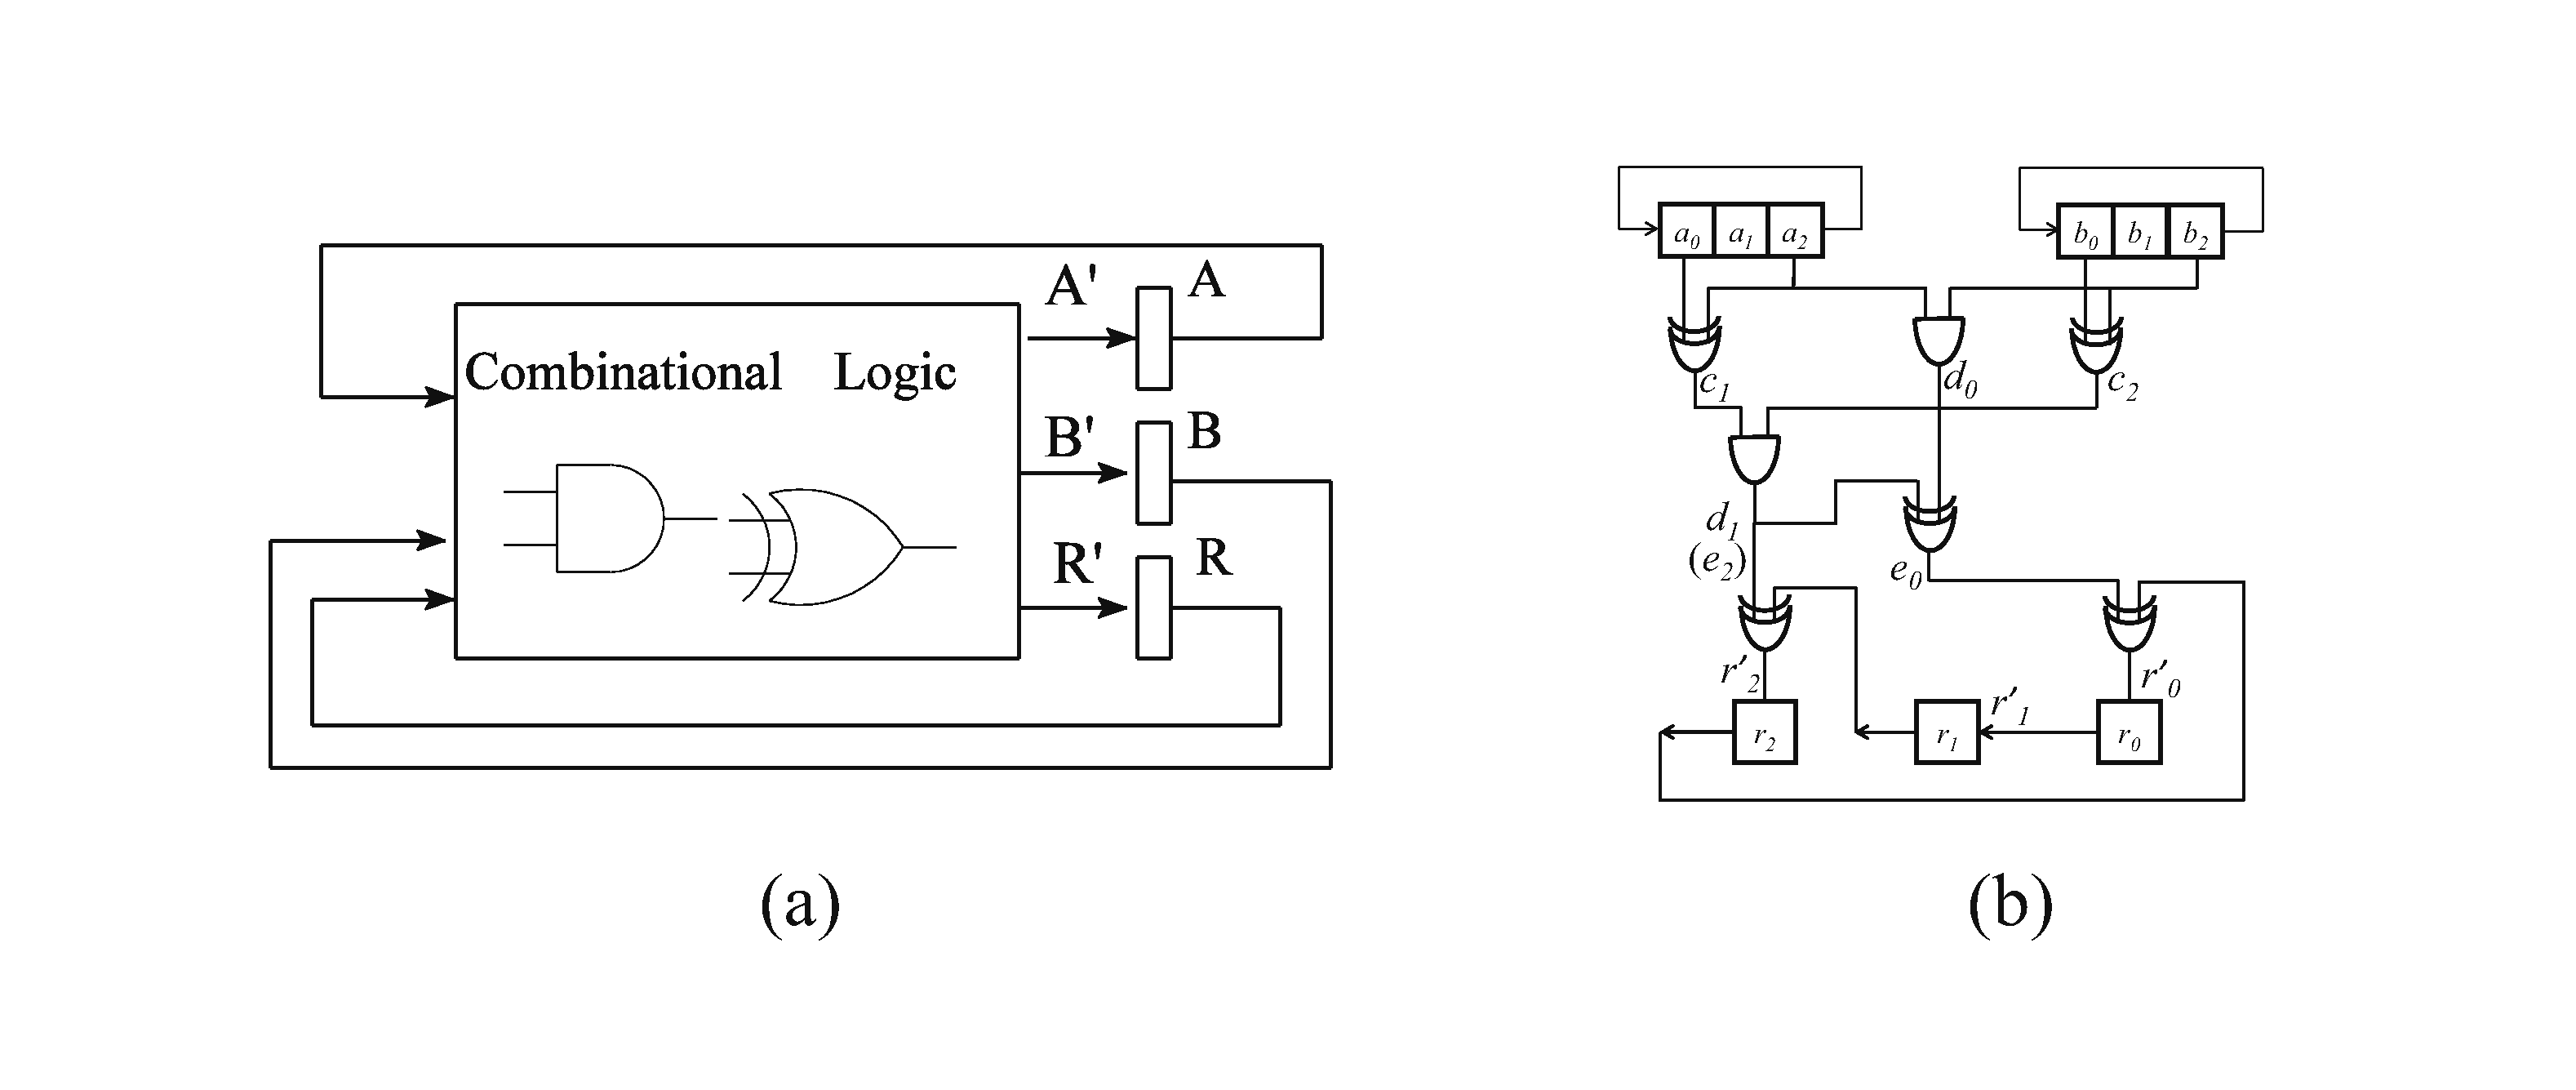
\includegraphics[width=4.5in]{./new_multi.eps}
% \vspace{-0.2in}
\caption{A 3-bit RH-SMPO and its Moore FSM model}
%\end{minipage}
\label{fig:RHmulti}}
\end{figure}

We follow  the typical sequential GF circuit model with word-level variables $A, B, R$
denoting {\it present states (PS)} and $A', B', R'$ denoting {\it next
  states (NS)} of the machine; where $A = \sum_{i=0}^{k-1} a_i \beta^{2^i}$
for the PS variables and $A' = \sum_{i=0}^{k-1} a_i'
\beta^{2^i}$ for NS variables, and so on.  Variables $R\ (R')$ correspond to those that 
store the result, and $A, B\ (A', B')$ store input operands. {\it E.g.,}
for a GF multiplier, $A_{init}, B_{init}$ (and $R_{init} =
0$) are the initial values (operands) loaded into the registers,  and
$R = \F(A_{init}, B_{init}) = A_{init} \times B_{init}$ is the final
result after $k$-cycles. Our approach aims to find this polynomial
representation for $R$.  

Each gate in the combinational logic is represented by a Boolean
polynomial. To 
this set of Boolean polynomials, we append the polynomials that define
the word-level to bit-level relations for PS and NS variables ($A =
\sum_{i=0}^{k-1} a_i \beta^{2^i}$). We denote this set of polynomials
as ideal $J = \langle 
f_1, \dots, f_s \rangle \subset \Fkk[x_1, \dots, x_d, R, R', A, A', B,
  B']$, where $x_1, \dots, x_d$ denote the bit-level (Boolean) variables
  of the circuit. The ideal of vanishing polynomials $J_0$ is also included, and
then the implicit FSM unrolling problem is setup for abstraction. 

The configurations of the flip-flops are the states of the
machine. {\it Since the set of states is a finite set of points, we
can consider it as the variety of an ideal related to the circuit
}. Moreover, since we are interested in
the {\it function encoded} by the state variables (over $k$-time
frames), we can {\it project this variety} on the word-level state
variables, starting from the initial state $A_{init}, B_{init}$.
Projection of varieties (geometry) corresponds to elimination ideals
(algebra), and can be analyzed via \Grobner bases. Therefore, we
employ a \Grobner basis computation with abstraction term order (ATO)\cite{timDAC}: we use a {\it lex term
  order} with {\it bit-level variables} 
$>$ {\it word-level NS outputs} $>$ {\it word-level PS inputs}. This
allows to eliminate all the bit-level variables 
%(corresponding to the combinational logic and the state variables),
%so as to 
and derives a representation only in terms of words. 
Consequently, $k$-successive \Grobner basis computations implicitly
unroll the machine, and provide word-level algebraic $k$-cycle
abstraction for $R'$ as $R' = \F(A_{init}, B_{init})$. 

Algorithm
\ref{alg:modified} describes our approach.  In the algorithm, $from_i$
and $to_i$ are polynomial ideals whose varieties are the valuations of
word-level variables $R, A, B$ and $R',A',B'$ in the $i$-th iteration;
and the notation ``$\setminus$'' signifies that the $NS$ in iteration
$(i)$ becomes the $PS$ in iteration $(i+1)$. Line 5 computes the Gr\"obner 
basis with the abstraction term order.  Line 6 computes the elimination 
ideal, eliminating the bit-level variables and representing the set of 
reachable states up to iteration $i$ in terms of the elimination ideal. 
These computations are analogous to those of image computations performed in FSM reachability. 
%The forward image
%$to^{i}$ is computed using \Grobner bases with ATO.

\vspace{-0.1in}
\IncMargin{1em}
\begin{algorithm}[hbt]
\SetAlgoNoLine
\LinesNumbered
 \KwIn{Circuit polynomial ideal $J$, vanishing ideal $J_0$, initial
   state ideal $R (=0), \mathcal{G}(A_{init}), \mathcal{H}(B_{init})$} 

  $from_0(R,A,B) = \langle R, \mathcal{G}(A_{init}), \mathcal{H}(B_{init})\rangle$\;
  $i = 0$\;
  \Repeat{$i == k$}
  {
  	$i \gets i + 1$\;
%	$to^i(R',A',B') \gets$  $GB( \langle J_{ckt}, J_0,
%    from^{i-1}(R,A,B)\rangle )$ with abstraction term order\;
	$G \gets$GB$( \langle J + J_0+ from_{i-1}(R,A,B) \rangle
    )$ with ATO\;
	$to_i(R',A',B')\gets G\cap \mathbb F_{2^k}[R',A',B',R,A,B]$\;
	$from_i \gets to_i(\{R,A,B\}\setminus \{R',A',B'\})$\;
  }
\Return{$from_k(R_{final})$}
\caption {Abstraction via implicit unrolling for Sequential GF circuit
  verification}
\label{alg:modified}
\end{algorithm}
\DecMargin{1em}
\vspace{-0.1in}
\begin{example}
\label{ex:RHSMPO}

We demonstrate our approach to verify the 3-bit RH-SMPO circuit of
Fig.\ref{fig:RHmulti}. The normal element $\beta$ in
$\mathbb{F}_{2^3}$ is known to be $\beta = \alpha^3$, where $\alpha$
is the primitive element. The circuit can be described with an ideal by translating
AND and XOR gates accordingly. For the first iteration:
\begin{align*}
J = &d_0+b_2\cdot a_2,
c_1+a_0+a_2,
c_2+b_0+b_2,
d_1+c_1\cdot c_2,\\
&e_0+d_0+d_1,
e_2+d_1,
r_0'+r_2+e_0,
r_1'+r_0,
r_2'+r_1+e_2,\\
&A+a_0\alpha^3+a_1\alpha^6+a_2\alpha^{12},
B+b_0\alpha^3+b_1\alpha^6+b_2\alpha^{12},\\
&R+r_0\alpha^3+r_1\alpha^6+r_2\alpha^{12},
R'+r_0'\alpha^3+r_1'\alpha^6+r_2'\alpha^{12};
\end{align*}
The last 4 polynomials are translated from the definition of word-level variables.
This represents ideal ``$J$" from line 5 in Algorithm
\ref{alg:modified}. ``$J_0$" is the ideal of vanishing polynomials in all bit-level
variables (e.g. $a_0^2-a_0$) and word-level variables (e.g. $A^8-A$). ``$from_{i-1}$"
represents the set of current states for iteration $i$.
In the first iteration, $from_0 = \{R, A_{init}+a_0\alpha^3+a_1\alpha^6+a_2\alpha^{12},
B_{init}+b_0\alpha^3+b_1\alpha^6+b_2\alpha^{12}\}$.

After the GB computation is performed with ATO, as line 6 in Algorithm \ref{alg:modified},
we find a polynomial in variables $R', A_{init}, B_{init}$ in $to_1 : 
R'+(\alpha^2) A_{init}^4 B_{init}^4+(\alpha^2+\alpha) A_{init}^4 B_{init}^2+(\alpha^2+\alpha) A_{init}^4 B_{init}+(\alpha^2+\alpha) A_{init}^2 B_{init}^4+(\alpha^2+\alpha+1) A_{init}^2 B_{init}^2+(\alpha^2) A_{init}^2 B_{init}+(\alpha^2+\alpha) A_{init} B_{init}^4+(\alpha^2) A_{init} B_{init}^2
$.

Line 7 in Algorithm \ref{alg:modified} simply replaces NS output $R'$ with PS output
$R$ in this example; so in second iteration $from_1 = \{
R'+(\alpha^2) A_{init}^4 B_{init}^4+(\alpha^2+\alpha) A_{init}^4 B_{init}^2+(\alpha^2+\alpha) A_{init}^4 B_{init}+(\alpha^2+\alpha) A_{init}^2 B_{init}^4+(\alpha^2+\alpha+1) A_{init}^2 B_{init}^2+(\alpha^2) A_{init}^2 B_{init}+(\alpha^2+\alpha) A_{init} B_{init}^4+(\alpha^2) A_{init} B_{init}^2
, A_{init}+a_2\alpha^3+a_0\alpha^6+a_1\alpha^{12},
B_{init}+b_2\alpha^3+b_0\alpha^6+b_1\alpha^{12}\}$. 

% By continue executing the loop,
Finally, after 3 iterations we obtain: $to_3 = \{ \mathbf{R'+A_{init}B_{init},}
~A_{init}+a_0'\alpha^3+a_1'\alpha^6+a_2'\alpha^{12},
~B_{init}+b_0'\alpha^3+b_1'\alpha^6+b_2'\alpha^{12}\}$
as the image. The final result is $from_3(R_{final}) = R_{final}+A_{init}\cdot
B_{init}$, which verifies the multiplier. 
\end{example}
Using our approach we successfully verified the function of an 100-bit RH-multiplier,
which implies its capability to handle the verification of large designs. The results
are published in \cite{myDATE}.